\documentclass[]{elsarticle} %review=doublespace preprint=single 5p=2 column
%%% Begin My package additions %%%%%%%%%%%%%%%%%%%
\usepackage[hyphens]{url}



\usepackage{lineno} % add
\providecommand{\tightlist}{%
  \setlength{\itemsep}{0pt}\setlength{\parskip}{0pt}}

\usepackage{graphicx}
\usepackage{booktabs} % book-quality tables
%%%%%%%%%%%%%%%% end my additions to header

\usepackage[T1]{fontenc}
\usepackage{lmodern}
\usepackage{amssymb,amsmath}
\usepackage{ifxetex,ifluatex}
\usepackage{fixltx2e} % provides \textsubscript
% use upquote if available, for straight quotes in verbatim environments
\IfFileExists{upquote.sty}{\usepackage{upquote}}{}
\ifnum 0\ifxetex 1\fi\ifluatex 1\fi=0 % if pdftex
  \usepackage[utf8]{inputenc}
\else % if luatex or xelatex
  \usepackage{fontspec}
  \ifxetex
    \usepackage{xltxtra,xunicode}
  \fi
  \defaultfontfeatures{Mapping=tex-text,Scale=MatchLowercase}
  \newcommand{\euro}{€}
\fi
% use microtype if available
\IfFileExists{microtype.sty}{\usepackage{microtype}}{}
\bibliographystyle{elsarticle-harv}
\usepackage{longtable}
\ifxetex
  \usepackage[setpagesize=false, % page size defined by xetex
              unicode=false, % unicode breaks when used with xetex
              xetex]{hyperref}
\else
  \usepackage[unicode=true]{hyperref}
\fi
\hypersetup{breaklinks=true,
            bookmarks=true,
            pdfauthor={},
            pdftitle={Mapping Flood-based Farming Systems with Bayesian networks.},
            colorlinks=false,
            urlcolor=blue,
            linkcolor=magenta,
            pdfborder={0 0 0}}
\urlstyle{same}  % don't use monospace font for urls

\setcounter{secnumdepth}{5}
% Pandoc toggle for numbering sections (defaults to be off)


% Pandoc header
\usepackage{setspace}\setstretch{1.5}
\usepackage[ruled,vlined,linesnumbered]{algorithm2e}
\usepackage{booktabs}
\usepackage{longtable}
\usepackage{array}
\usepackage{multirow}
\usepackage{wrapfig}
\usepackage{float}
\usepackage{colortbl}
\usepackage{pdflscape}
\usepackage{tabu}
\usepackage{threeparttable}
\usepackage{threeparttablex}
\usepackage[normalem]{ulem}
\usepackage{makecell}
\usepackage{xcolor}



\begin{document}
\begin{frontmatter}

  \title{Mapping Flood-based Farming Systems with Bayesian networks.}
    \author[KU,ICRAF]{Issoufou, Liman Harou\corref{Corresponding Author}}
   \ead{issoufoul@gmail.com; L.issoufou@cgiar.org} 
    \author[INRES]{Cory Whitney}
   \ead{cory.whitney@uni-bonn.de} 
    \author[KU]{James Kungu}
   \ead{kungu.james@ku.ac.ke} 
    \author[INRES]{Eike Luedeling}
   \ead{luedeling@uni-bonn.de} 
      \address[KU]{Kenyatta University, Department of Environmental Sciences, P.O. Box 43844 00100 Nairobi, Kenya}
    \address[ICRAF]{World Agroforestry Centre (ICRAF), United Nations Avenue, Gigiri, P.O. Box 30677-00100, Nairobi, Kenya}
    \address[INRES]{University of Bonn, Department of Horticultural Sciences, Auf dem Hügel 6, D-53121, Bonn, Germany}
    \address[ZEF]{Center for Development research (ZEF), University of Bonn, Genscherallee 3, D-53113, Bonn, Germany}
    
  \begin{abstract}
  Many actors in agricultural research, development and policy require accurate information on the spatial extents of cropping and farming practices. While remote sensing provides venues for obtaining such information, it is often difficult to distinguish between agricultural practices which can be quite similar in their spectral signatures. This can easily lead to misclassification by traditional algorithms. We addressed this limitation by combining traditional remote sensing techniques with probabilistic reasoning engines informed by expert knowledge to map flood-based farming systems, an important form of agricultural production employed by farmers in regions with seasonal water surplus. Flood-based farming systems were mapped across Kisumu County in Kenya and the Tigray region in Ethiopia using a model of causality. While the two areas present noticeable differences in terms of their hydrology, vegetation, or the practice of agronomic flooding, these relevant aspects for mapping flood-based farming systems are mostly stochastic in space and time, which makes it difficult to provide a generalizable characterization of the practice using precise quantifiers. Recognizing this aspect, the causal model described in this paper considers uncertainties across expert-based estimates to provide quantitative assessment of the overall uncertainty in the final output. To account for the effect of specific geographic settings, we used Bayesian networks informed by expert knowledge to characterize these settings. Three years (2014-2016) of processed MODIS VI data were acquired in the forms of normalized difference spectral indices which were used as proxies for estimating various spatial metrics relevant for flood-based farming systems detection. The spatial metrics along with other non-spatial data derived from expert judgement were used as nodes to feed the Bayesian networks. Results were transparently generated in the form of intermediary prior spatial maps for specific metrics to ultimately be aggregated into final posterior maps of plausible areas for flood-based farming along with their spatially explicit uncertainties. We demonstrate that spatially explicit information can be derived from remote sensing data as fuzzy linguistic quantifiers which are suitable for representing node states in Bayesian networks. When such metrics are available, Bayesian networks are useful tools for incorporating uncertainties when mapping complex systems in a context of limited and uncertain information. The causal probabilistic reasoning embedded in the approach achieved a remarkably accurate result in both settings where 60 to 100\% of various flood-based farming system fields sampled from different locations were correctly mapped with high chance of being suitable for the practice.
  \end{abstract}
  
 \end{frontmatter}

\hypertarget{introduction}{%
\section*{Introduction}\label{introduction}}
\addcontentsline{toc}{section}{Introduction}

\hypertarget{section_1}{%
\section{Study area}\label{section_1}}

\begin{figure}[!h]

{\centering 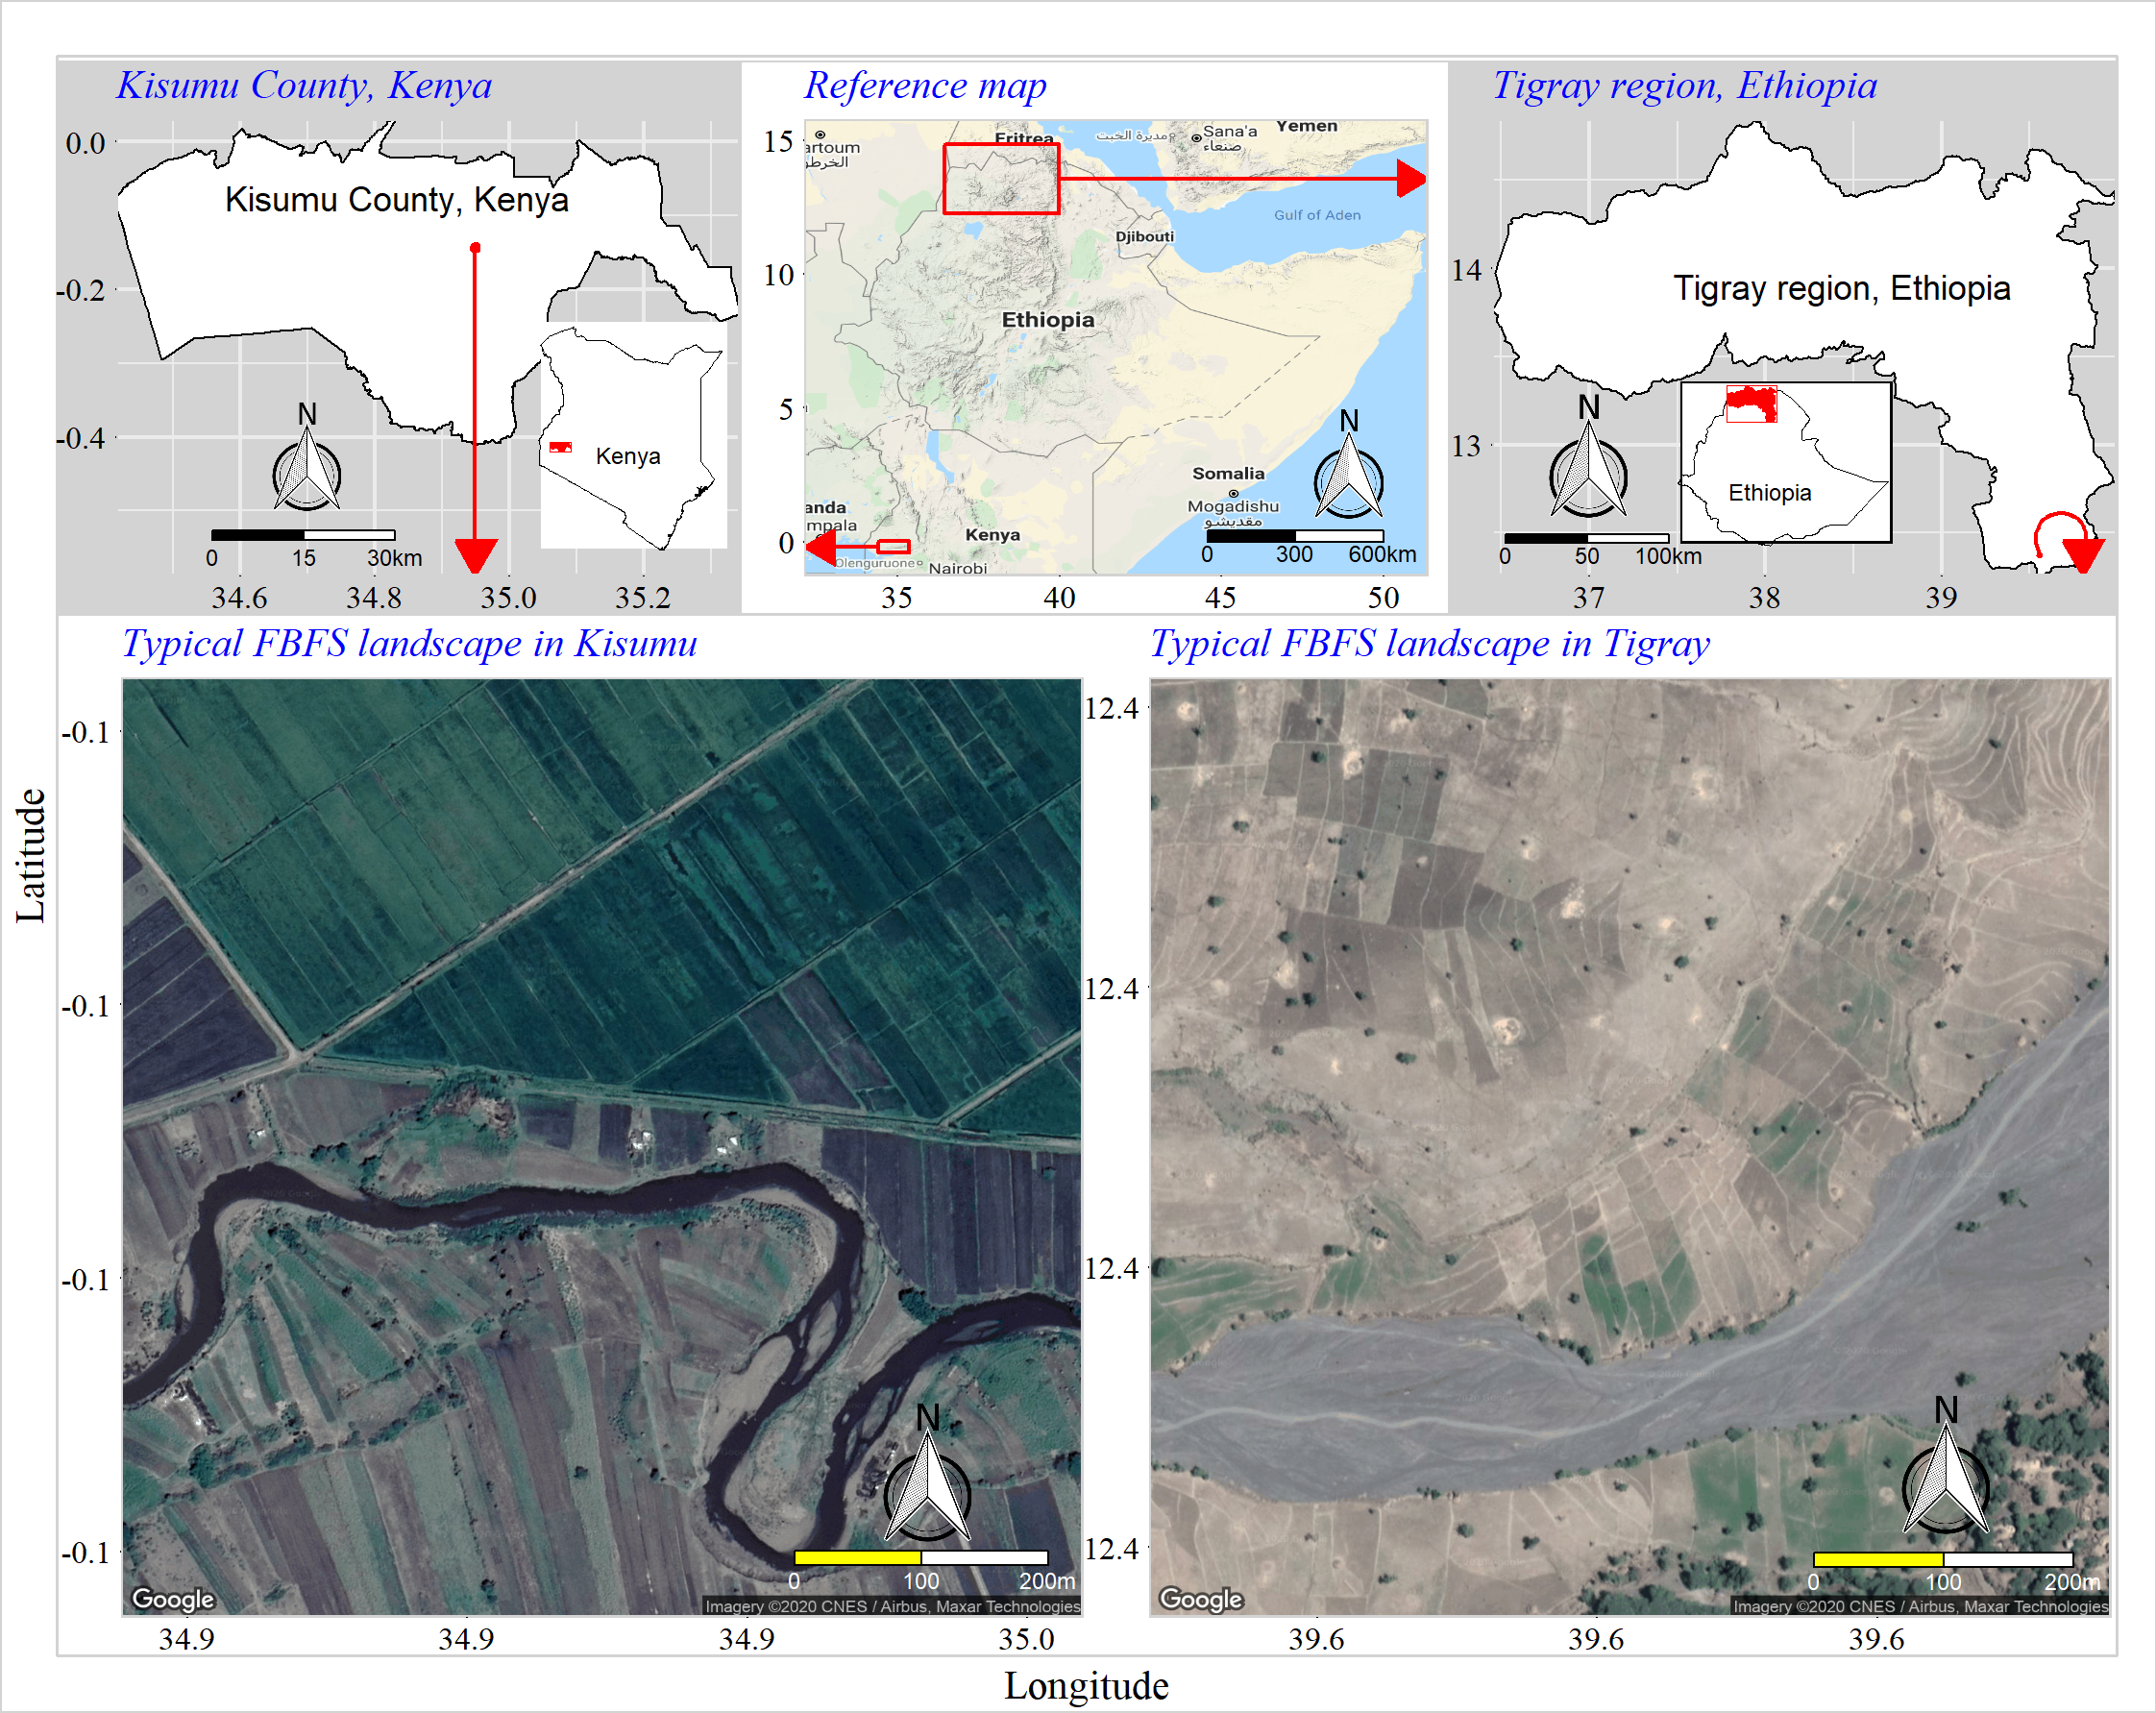
\includegraphics[width=1\linewidth,]{figures/study_area_map} 

}

\caption{Typical flood-based farming systems landscapes found in Tigray region of Ethiopia and Kisumu County in Kenya.}\label{fig:fig1}
\end{figure}

\hypertarget{section_2}{%
\section{Material and methods}\label{section_2}}

\hypertarget{section_2_1}{%
\subsection{Conceptual framework}\label{section_2_1}}

\begin{figure}[!h]

{\centering \includegraphics[width=1\linewidth,]{Mapping_FBFS_files/figure-latex/fig1-plot-1} 

}

\caption{Conceptual framework for mapping FBFS in Kisumu County, Kenya and Tigray region, Ethiopia.}\label{fig:fig2}
\end{figure}

\hypertarget{section_2_2}{%
\subsection{Sensor Characteristics}\label{section_2_2}}

\hypertarget{section_2_3}{%
\subsection{Data acquisition and pre-processing}\label{section_2_3}}

\hypertarget{section_2_3_1}{%
\subsubsection{The BNs}\label{section_2_3_1}}

\begin{figure}[!h]

{\centering \includegraphics[width=1\linewidth,]{Mapping_FBFS_files/figure-latex/fig2-plot-1} 

}

\caption{Bayesian Network describing the causal reasoning used for mapping FBFS in Kisumu, Kenya.}\label{fig:fig3}
\end{figure}

\begin{table}

\caption{\label{tab:tab1}List of normalized difference spectral indices (NDSI) used for mapping FBFS in Kisumu County, Kenya.}
\centering
\resizebox{\linewidth}{!}{
\begin{tabular}[t]{>{\bfseries}llll}
\toprule
\textbf{ } & \textbf{Bands} & \textbf{Spectral range} & \textbf{Full name}\\
\midrule
NDVI & B2, B1 & (NIR – VISRed)/(NIR + RED) & Normalized Difference Vegetation Index (Rouse, 1973)\\
NDFI & B1, B6 & (NIR - SWIR1) / (NIR + SWIR1) & Normalized Difference Flood Index (Boschetti, 2014)\\
NDII6 & B2, B6 & (NIR2 - SWIR1) / (NIR2 + SWIR1) & Normalized Difference Infrared Index - Band 6 (Hunt, 1989)\\
NDII7 & B2, B7 & (NIR2 - SWIR2) / (NIR2 + SWIR2) & Normalized Difference Infrared Index - Band 7 (Hunt, 1989)\\
GAO MDWI & B2, B5 & (NIR2 - NIR5) / (NIR2 + NIR5) & Normalized Difference Water Index (NDWI) (GAO, 1996)\\
\addlinespace
McFeeters MDWI & B4, B2 & (VIS4 – NIR2) / (VIS4 + NIR2) & Normalized Difference Water Index (NDWI) (McFeeters, 1996)\\
\bottomrule
\end{tabular}}
\end{table}

\hypertarget{section_2_3_2}{%
\subsubsection{Spatial data}\label{section_2_3_2}}

\hypertarget{section_2_4}{%
\subsection{Making sense of data in specific contexts}\label{section_2_4}}

\hypertarget{section_2_5}{%
\subsection{Deriving spatial data nodes}\label{section_2_5}}

\hypertarget{section_2_5_1}{%
\subsubsection{General multi-layer procedure applied to time series data}\label{section_2_5_1}}

dddddddddddddddddddd hhhhhhhhhhhhhhhhhhhhhhhh

\begin{algorithm}[H]
\SetKw{KwBy}{by}
\DontPrintSemicolon
\SetAlgoLined
\KwResult{a spatially explicit quantitative representation of variable states using probability}
\SetKwInOut{Input}{Input}\SetKwInOut{Output}{Output}
\Input{NDSI time series stack}
\Output{a raster stack where each layer represents one of the variable states}
\BlankLine
\For{$each\;layer\;in\;the\;time\;series$}{
    compute Whisker ranges\;
    \For{$each\;Whisker\;range$}{
        \eIf{cell value belongs to the Whisker range}{
        recode the cell value to 1\;
    }{
        recode the cell value to 0\;
    }
    compute the probability of getting 1
}
}
\caption{make pixel states}
\end{algorithm}

\begin{equation} 
P(p_i \in range_j) = \frac{n_{p_i \in range_j}}{N}
\label{eq:eq1}
\end{equation}

Where \(P(p_i \in range_j)\) is the probability of the pixel \(p_i\) belonging to the range \(range_j\), \(n_{p_i \in range_j}\) is the number of time the pixel \(p_i\) belonged to the range \(range_j\), and \(N\) is the sample space (total size of the time series).

nnnnnnnnnn nnnnnnnnn nn nnnnnnnnnnnnnnn nnnnnnnnnnn nnnnnnnnnnnnnnnnnnnnnnnnnnn nnnnnnnnnnnnnnnnnnnnnnnnnnnnn nnnnnnnnnnnnnnnnnnnnnnnnnnn nnnnnnnnnnnnnn nnnnnnnnnnnnnnnnnnnnnnnnnnnnnnnnnnnnnnn nnnnnnnnnnnnnnnnnnnnnnnnnnnnnnnnnn nnnnnnnnnnnnnnnnnnnnnnnnnnnnnnn nnnnnnnnnnnnnnnnnnn nnnnnnnnnnnnnnnnnn nnnnnnnn n n nnnnnnnnnnnnnnnn nnnnnnnnnnnnnnnnnnnnnnnnnnnnnn

nnnnnnnnnn nnnnnnnnn nn nnnnnnnnnnnnnnn nnnnnnnnnnn nnnnnnnnnnnnnnnnnnnnnnnnnnn nnnnnnnnnnnnnnnnnnnnnnnnnnnnn nnnnnnnnnnnnnnnnnnnnnnnnnnn nnnnnnnnnnnnnn nnnnnnnnnnnnnnnnnnnnnnnnnnnnnnnnnnnnnnn nnnnnnnnnnnnnnnnnnnnnnnnnnnnnnnnnn nnnnnnnnnnnnnnnnnnnnnnnnnnnnnnn nnnnnnnnnnnnnnnnnnn nnnnnnnnnnnnnnnnnn nnnnnnnn n n nnnnnnnnnnnnnnnn nnnnnnnnnnnnnnnnnnnnnnnnnnnnnn

nnnnnnnnnn nnnnnnnnn nn nnnnnnnnnnnnnnn nnnnnnnnnnn nnnnnnnnnnnnnnnnnnnnnnnnnnn nnnnnnnnnnnnnnnnnnnnnnnnnnnnn nnnnnnnnnnnnnnnnnnnnnnnnnnn nnnnnnnnnnnnnn nnnnnnnnnnnnnnnnnnnnnnnnnnnnnnnnnnnnnnn nnnnnnnnnnnnnnnnnnnnnnnnnnnnnnnnnn nnnnnnnnnnnnnnnnnnnnnnnnnnnnnnn nnnnnnnnnnnnnnnnnnn nnnnnnnnnnnnnnnnnn nnnnnnnn n n nnnnnnnnnnnnnnnn nnnnnnnnnnnnnnnnnnnnnnnnnnnnnn

\begin{algorithm}[H]
\SetKw{KwBy}{by}
\DontPrintSemicolon
\SetAlgoLined
\KwResult{a spatially explicit qualitative representation of variable states using common language}
\SetKwInOut{Input}{Input}\SetKwInOut{Output}{Output}
\Input{NDSI time series stack}
\Output{a raster layer where pixels are represented using relative fuzzy linguistic quantifiers}
\BlankLine
\textbf{do} algorithm 1: make pixel states\ \label{lst:line:s1}\;
\For{$each\;pixel$}{
        \eIf{the pixel has one single maximum for all layers}{
        assign to the pixel the position of the layer (corresponding to a Whisker range as in the stack generated at step~\ref{lst:line:s1} and mapping to a linguistic quantifier) holding that maximum (probability) value \;
    }{
        assign NA to the pixel\ \label{lst:line:s2};
    }
    \For{$each\;pixel\;holding\;NA\;in\;the\;layer\;(generated\;after\;step~\ref{lst:line:s2})$}{
        \eIf{the pixel has one single maximum for all neighbours in the 8 ways connectedness}{
        fill it with that maximum value \;
        }{
        leave the pixel value as NA\ \label{lst:line:s13};
        }
            get the position of the remaining pixel holding after step~\ref{lst:line:s13} \;
            extract all pixel values at the positions in step~\ref{lst:line:s13} from the stack generated at step~\ref{lst:line:s1} \label{lst:line:s14}\;
            fit a classification regression tree model to the extracted data in step~\ref{lst:line:s14} \label{lst:line:s15}\;
            predict the remaining pixels holding NA after step~\ref{lst:line:s13} using the model developed at step~\ref{lst:line:s15}
    }
}
\caption{compile pixel states}
\end{algorithm}

\hypertarget{section_2_5_2}{%
\subsubsection{General procedure applied to single-layer data}\label{section_2_5_2}}

\hypertarget{section_2_5_3}{%
\subsubsection{Specific procedure used for spatial data generation}\label{section_2_5_3}}

\hypertarget{II}{%
\section{Results}\label{II}}

\hypertarget{section_3_1}{%
\subsection{Spatio-temporal analysis of water and vegetation in Kisumu County, Kenya}\label{section_3_1}}

\begin{figure}[!h]

{\centering 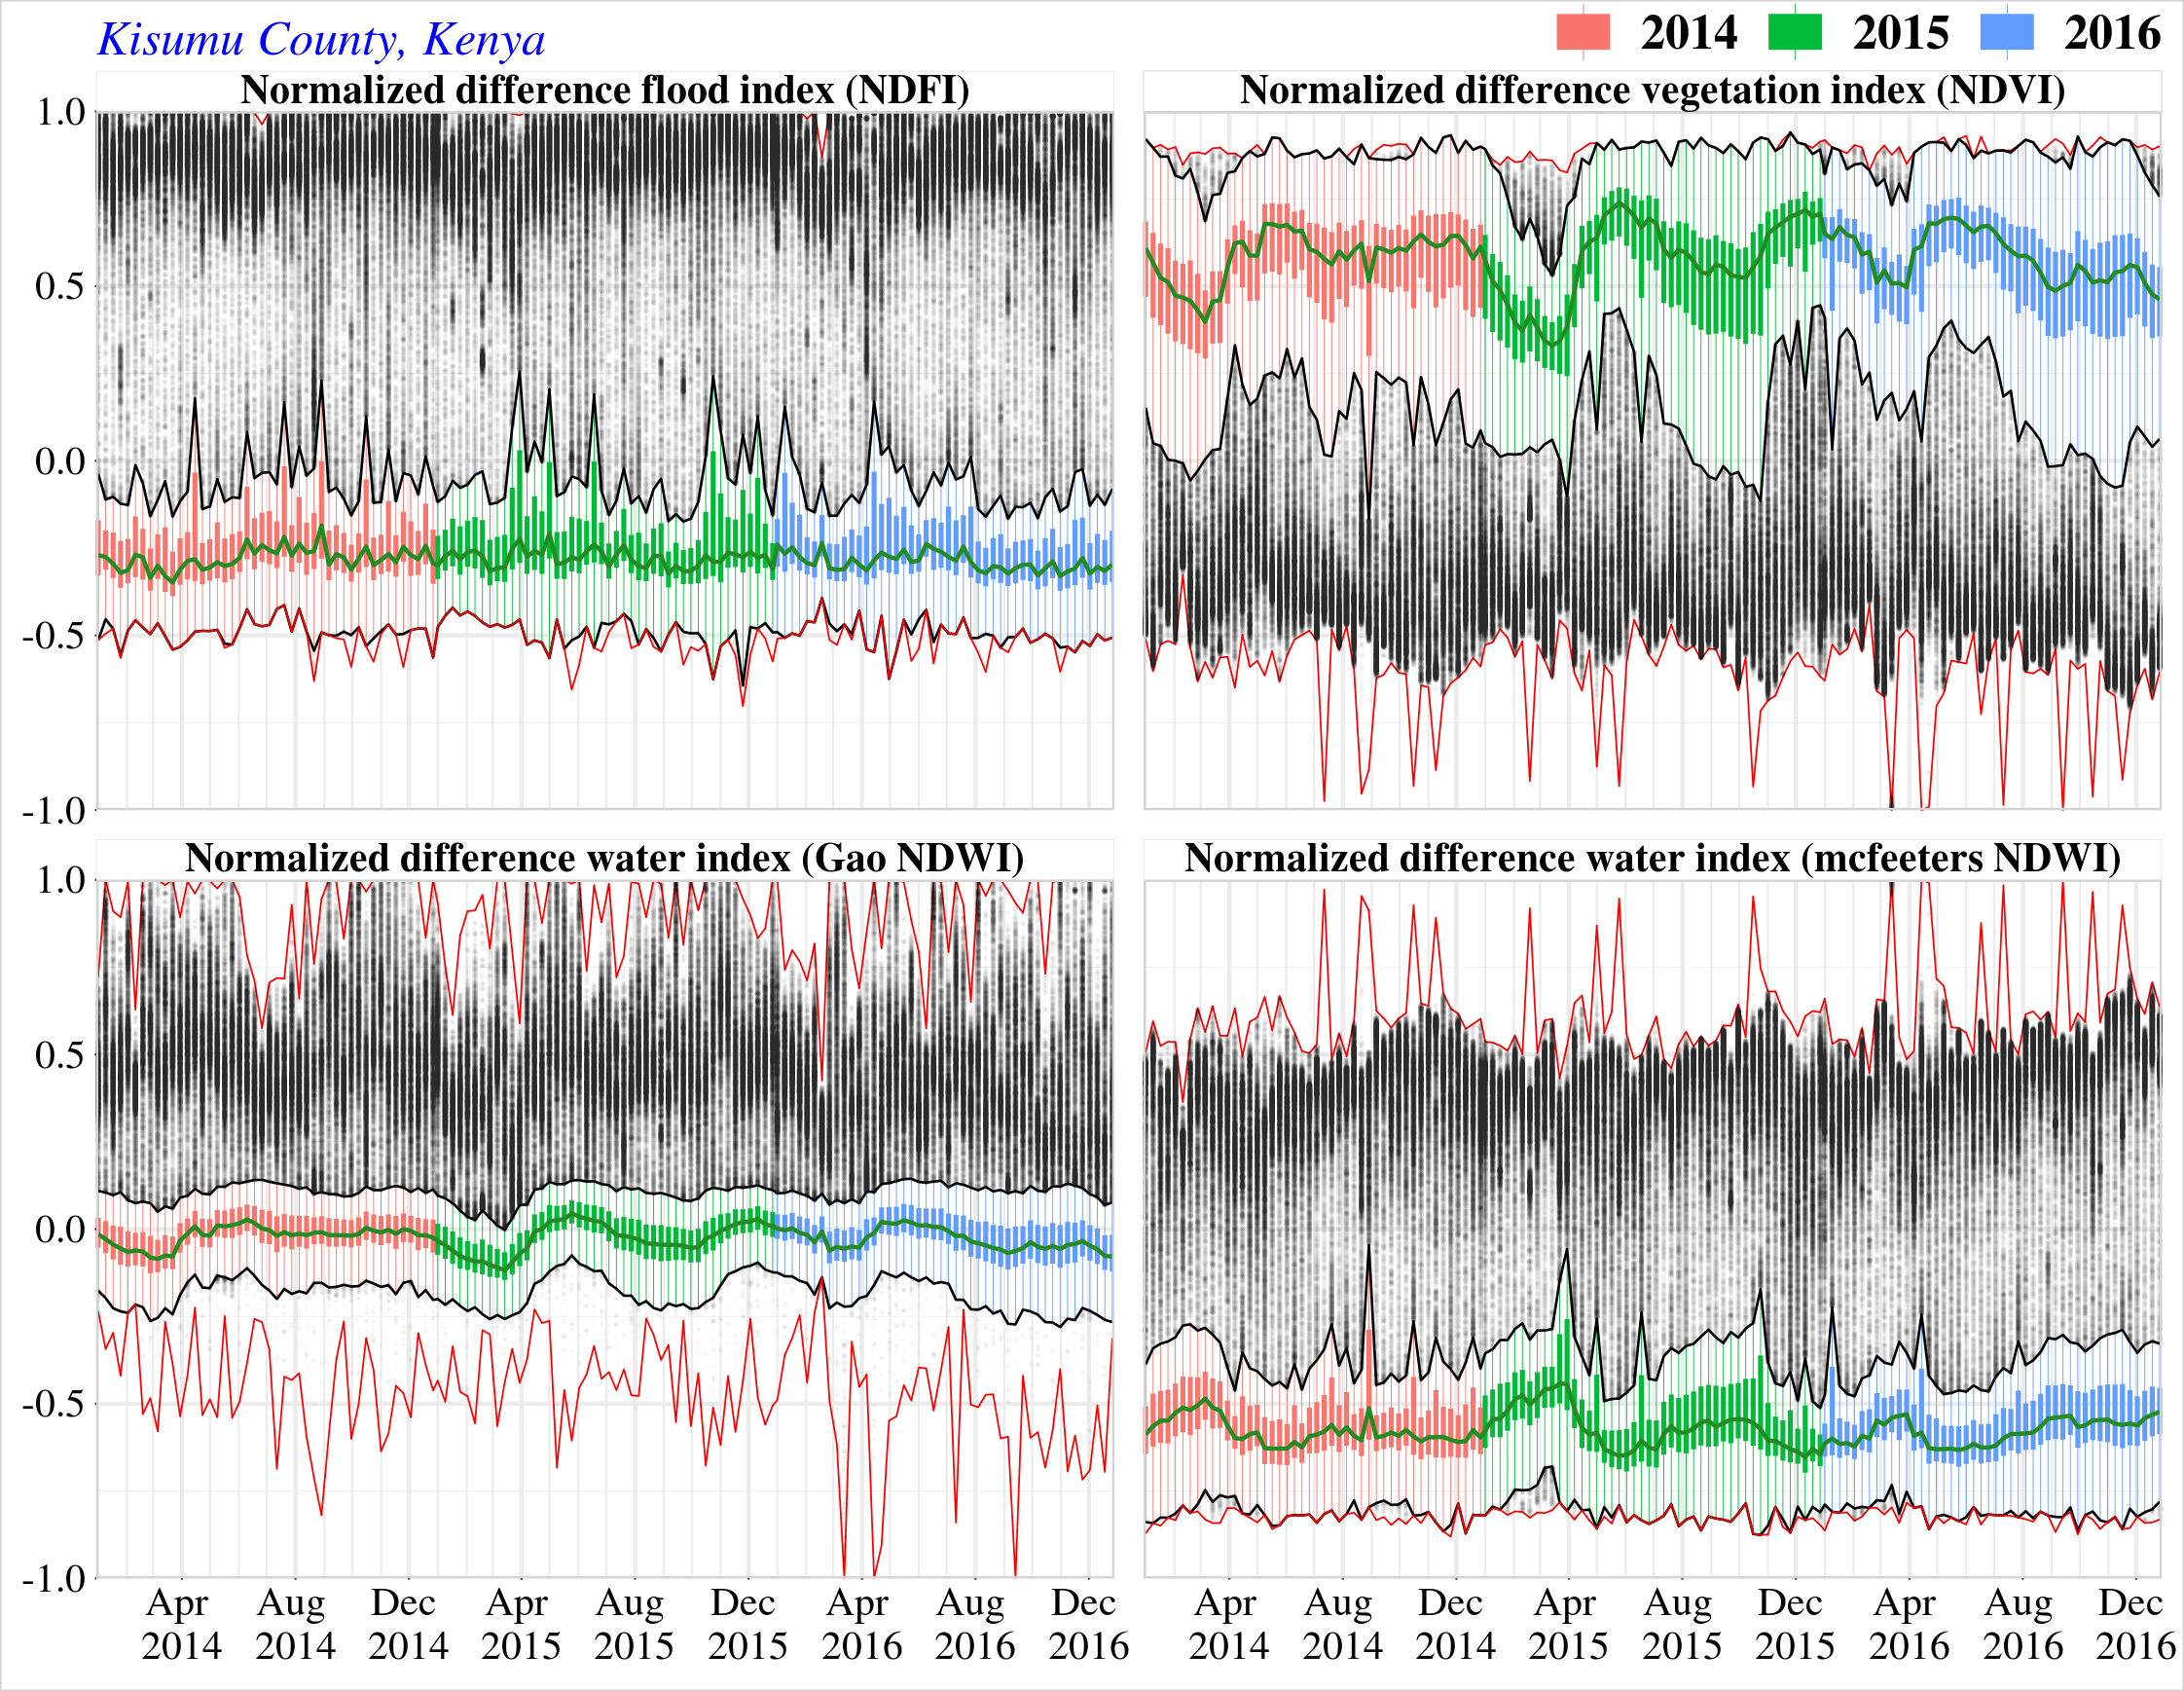
\includegraphics[width=1\linewidth,]{figures/seasonal_ranges_plot} 

}

\caption{Temporal variability in water and vegetation in Kisumu county, Kenya.}\label{fig:fig4}
\end{figure}

\begin{figure}[!h]

{\centering 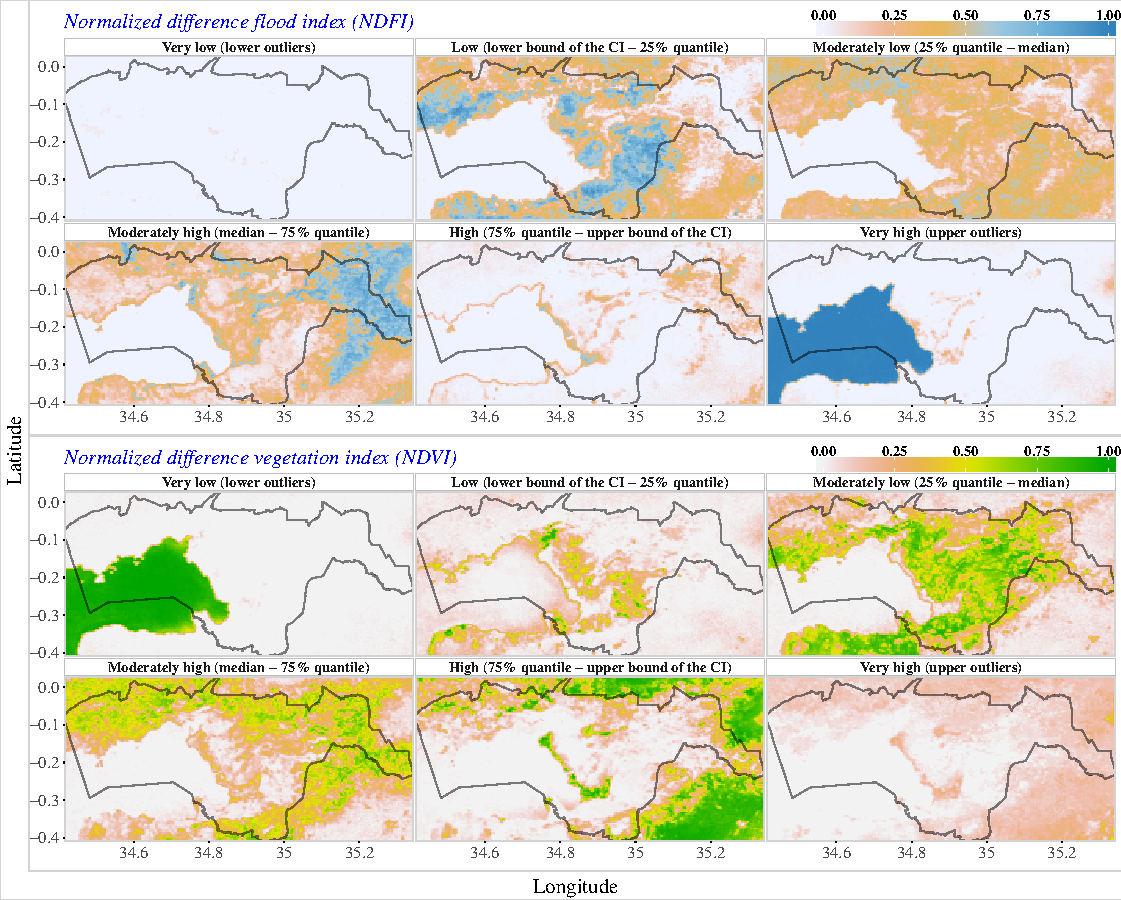
\includegraphics[width=1\linewidth,]{figures/veg_water_states_plot} 

}

\caption{Discrete states of vegetation and water in Kisumu county, Kenya.}\label{fig:fig5}
\end{figure}

\hypertarget{section_3_2}{%
\subsection{FBFS-relevant metrics}\label{section_3_2}}

\hypertarget{section_3_2_1}{%
\subsubsection{Prior distribution of FBFS-relevant metrics}\label{section_3_2_1}}

\begin{figure}[!h]

{\centering 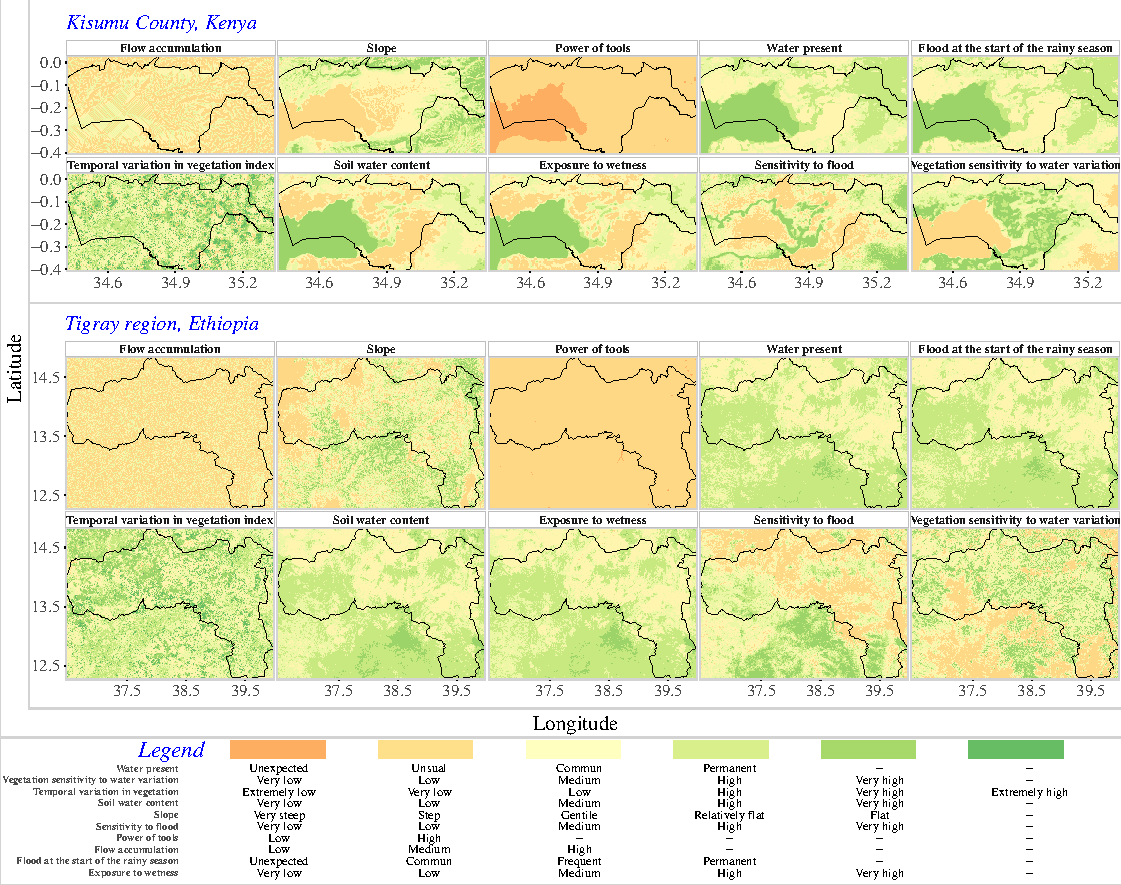
\includegraphics[width=1\linewidth,]{figures/prior_plot} 

}

\caption{Prior maps of differents spatial data used to feed the BNs for mapping FBFS in Kisumu county, Kenya and Tigray region, Ethiopia.}\label{fig:fig6}
\end{figure}

\hypertarget{section_3_2_2}{%
\subsubsection{Posterior distribution of FBFS-relevant metrics}\label{section_3_2_2}}

\begin{figure}[!h]

{\centering 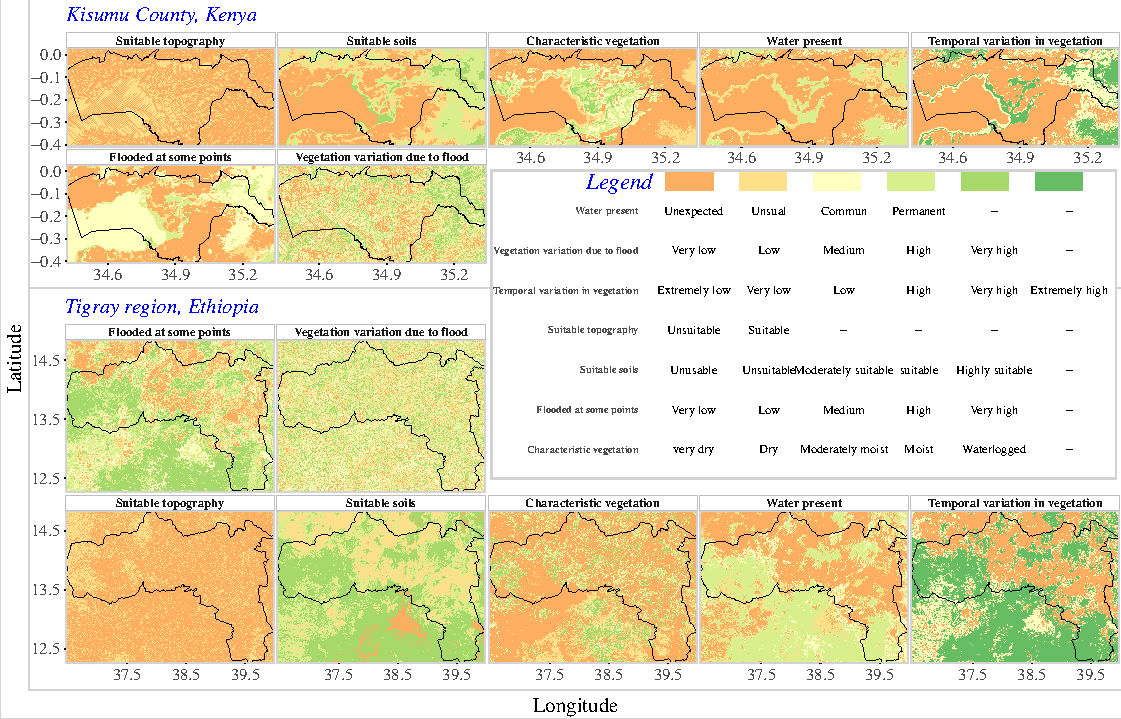
\includegraphics[width=1\linewidth,]{figures/posterior_plot} 

}

\caption{Posterior maps of differents spatial data used to feed the BNs for mapping FBFS in Kisumu county, Kenya and Tigray region, Ethiopia.}\label{fig:fig7}
\end{figure}

\hypertarget{section_3_2_3}{%
\subsubsection{Uncertainty of FBFS-relevant metrics}\label{section_3_2_3}}

\begin{figure}[!h]

{\centering 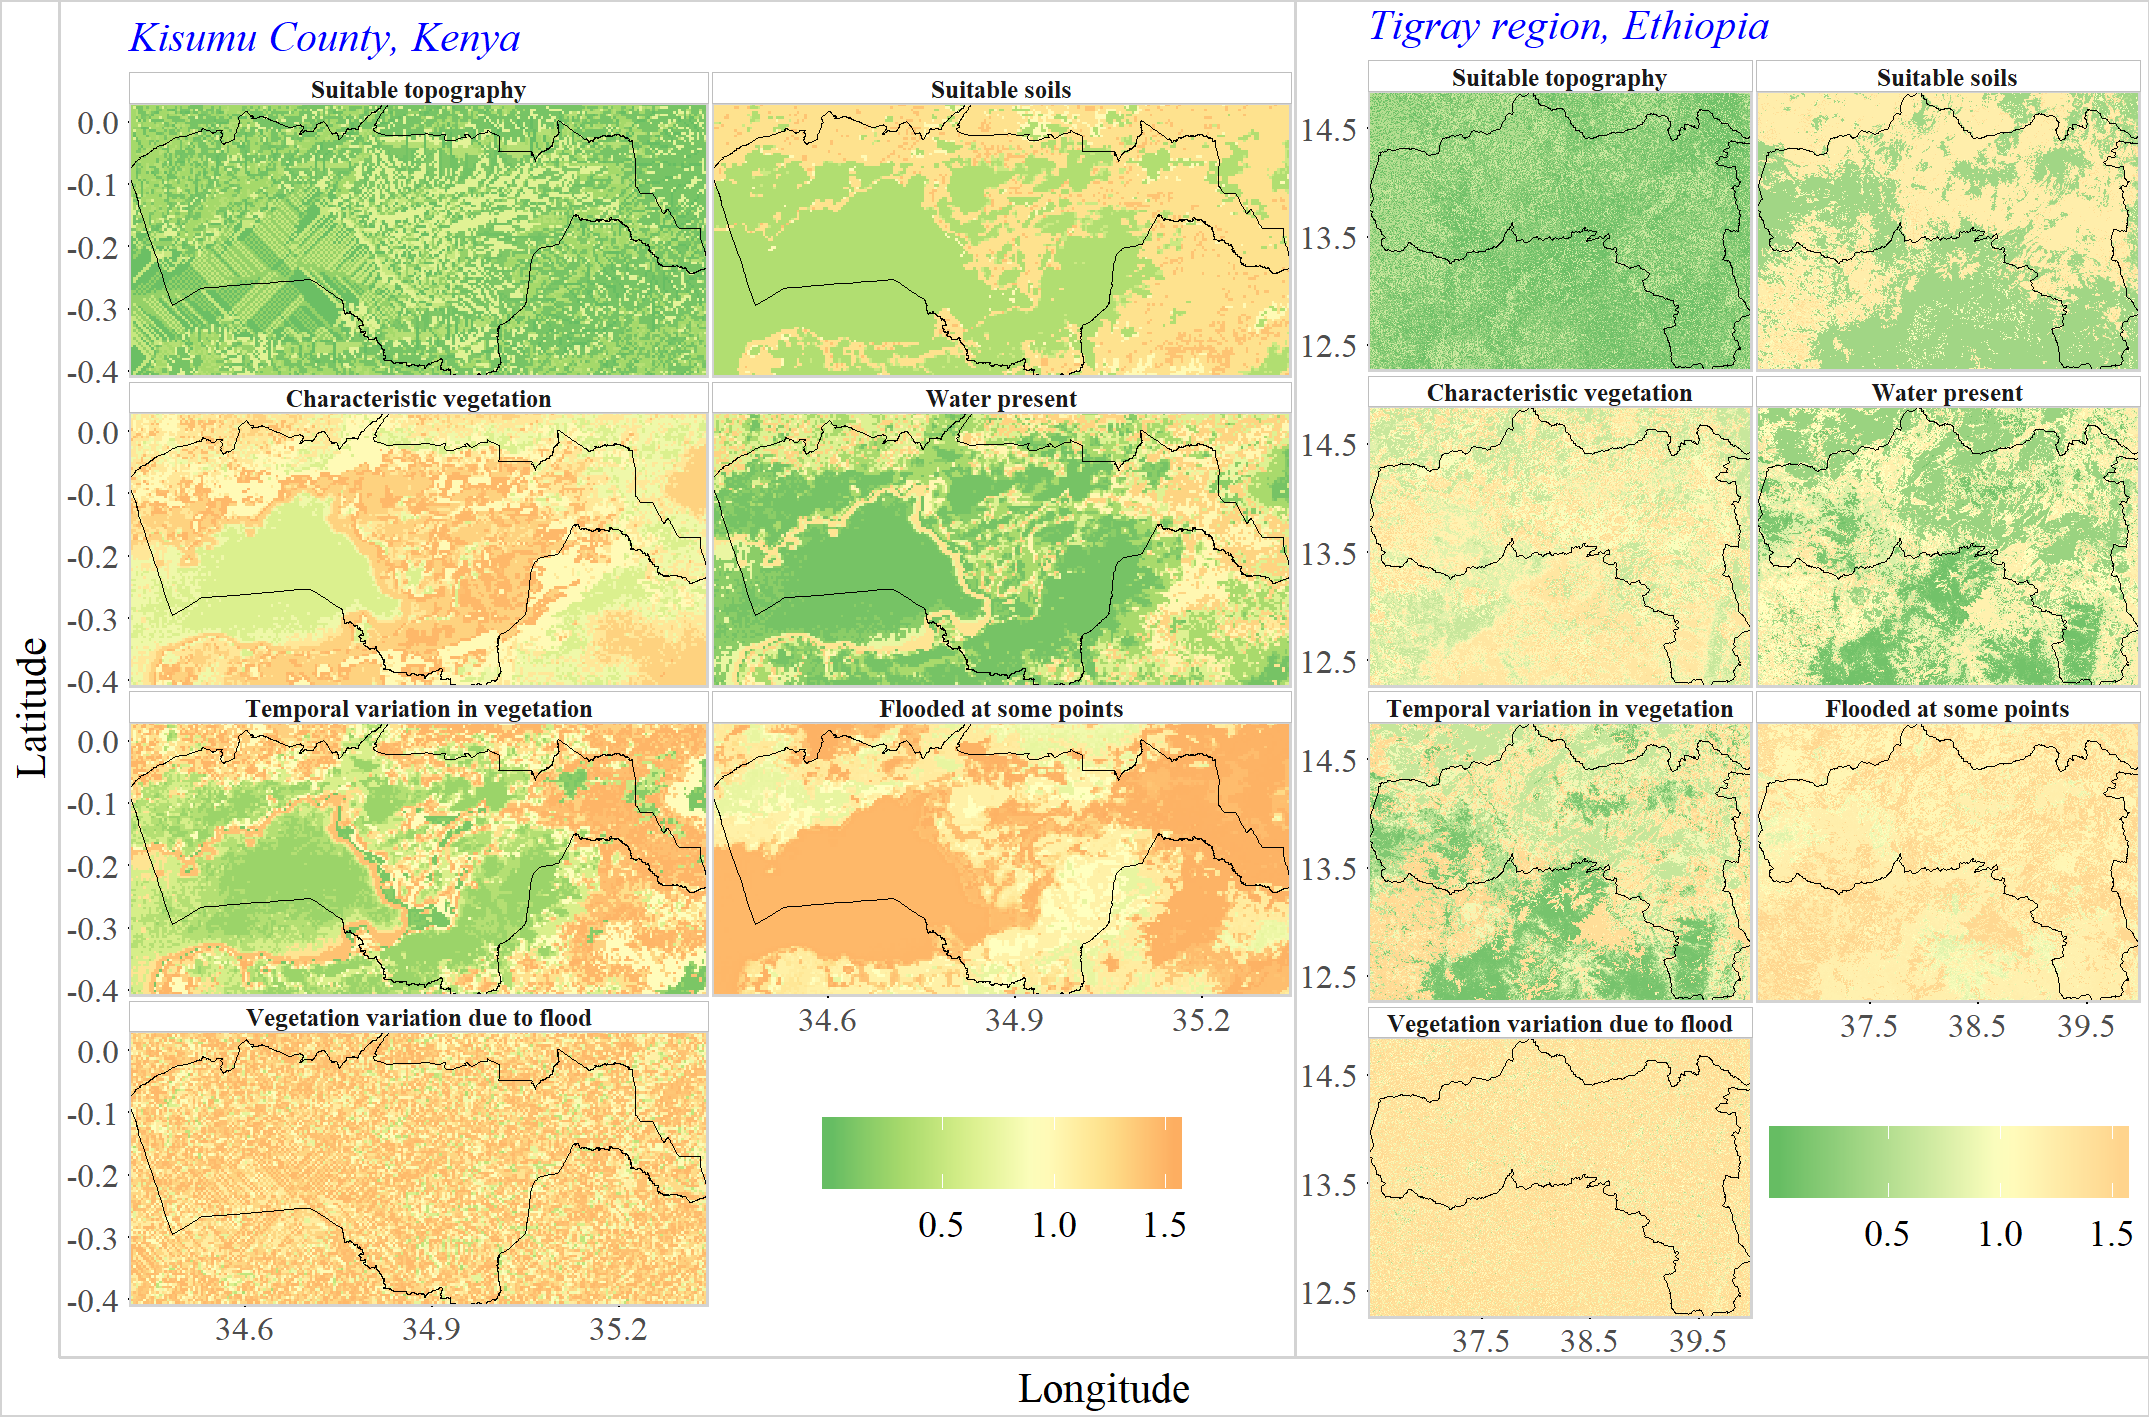
\includegraphics[width=1\linewidth,]{figures/uncertainty_plot} 

}

\caption{Uncertainty maps of differents spatial data used to feed the BNs for mapping FBFS in Kisumu county, Kenya and Tigray region, Ethiopia.}\label{fig:fig8}
\end{figure}

\hypertarget{section_3_3}{%
\subsection{FBFS potential in Kisumu County, Kenya and Tigray region, Ethiopia}\label{section_3_3}}

\begin{figure}[!h]

{\centering 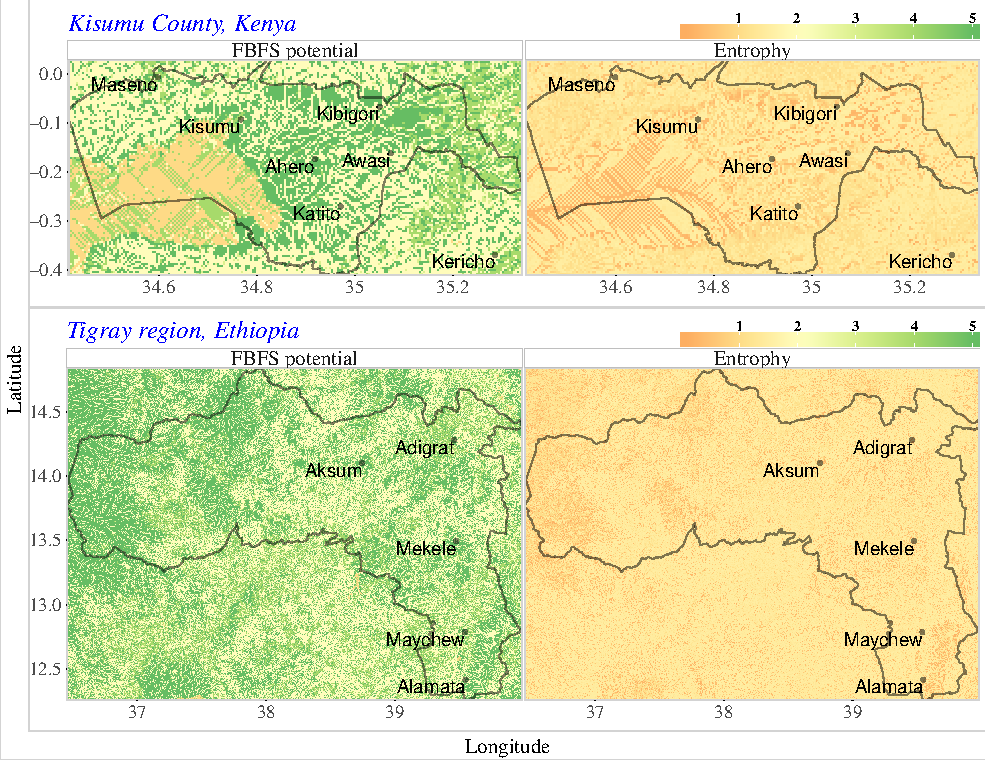
\includegraphics[width=1\linewidth,]{figures/FBFS_plot} 

}

\caption{Potential areas for FBFS and associated uncertainity in Kisumu County, Kenya and Tigray region, Ethiopia.}\label{fig:fig9}
\end{figure}

\begin{table}

\caption{\label{tab:tab5}Spatial coverage of FBFS in Kisumu County, Kenya and Tigray region, Ethiopia.}
\centering
\resizebox{\linewidth}{!}{
\begin{tabular}[t]{>{\bfseries}llllll}
\toprule
\textbf{ } & \textbf{Highly unlikely} & \textbf{Unlikely} & \textbf{Possible} & \textbf{Likely} & \textbf{Highly likely}\\
\midrule
Kisumu & 379.7
(14.2\%) & 1033.1
(38.8\%) & 30.2
(1.1\%) & 285.4
(10.7\%) & 936.5
(35.1\%)\\
Tigray & 20.8
(0.0\%) & 22727.9
(43.2\%) & 831.3
(1.6\%) & 6710.1
(12.8\%) & 22228.1
(42.3\%)\\
\bottomrule
\end{tabular}}
\end{table}

\hypertarget{section_3_4}{%
\subsection{Accuracy assessment}\label{section_3_4}}

\begin{table}

\caption{\label{tab:tab3}Prediction accuracy of a spatially explicit bayesian network used for mapping FBFS in Kisumu County, and Tigray region, Ethiopia.}
\centering
\resizebox{\linewidth}{!}{
\fontsize{6}{8}\selectfont
\begin{tabular}[t]{>{\bfseries}lllllll}
\toprule
\textbf{Study area} & \textbf{Validation sample} & \textbf{Highly unlikely} & \textbf{Unlikely} & \textbf{Possible} & \textbf{Likely} & \textbf{Highly likely}\\
\midrule
 & Bare lands & 66.7\% & 33.3\% & 0.0\% & 0.0\% & 0.0\%\\
\cmidrule{2-7}
 & FBFS Fields & 0.0\% & 0.0\% & 0.0\% & 0.0\% & 100.0\%\\
\cmidrule{2-7}
 & Forests & 0.0\% & 100.0\% & 0.0\% & 0.0\% & 0.0\%\\
\cmidrule{2-7}
 & Irrigated agricultural fields & 0.0\% & 20.5\% & 2.3\% & 2.3\% & 75.0\%\\
\cmidrule{2-7}
 & Rainfed agricultural fields & 0.0\% & 80.0\% & 0.0\% & 0.0\% & 20.0\%\\
\cmidrule{2-7}
 & Riperian forests & 0.0\% & 0.0\% & 0.0\% & 0.0\% & 100.0\%\\
\cmidrule{2-7}
 & Settlements & 0.0\% & 63.6\% & 0.0\% & 27.3\% & 9.1\%\\
\cmidrule{2-7}
 & Vegetated plateaux & 0.0\% & 88.9\% & 0.0\% & 0.0\% & 11.1\%\\
\cmidrule{2-7}
\multirow{-9}{*}{\raggedright\arraybackslash Kisumu} & Water bodies & 65.0\% & 7.1\% & 0.0\% & 27.9\% & 0.1\%\\
\cmidrule{1-7}
 & Bare lands & 0.0\% & 62.3\% & 0.6\% & 2.6\% & 34.4\%\\
\cmidrule{2-7}
 & FBFS fields & 0.0\% & 24.5\% & 0.0\% & 1.9\% & 73.6\%\\
\cmidrule{2-7}
 & Forests & 0.0\% & 77.8\% & 0.0\% & 11.1\% & 11.1\%\\
\cmidrule{2-7}
 & Irrigated agricultural fields & 0.0\% & 65.4\% & 0.0\% & 0.0\% & 34.6\%\\
\cmidrule{2-7}
 & Rainfed agricultural fields & 0.0\% & 100.0\% & 0.0\% & 0.0\% & 0.0\%\\
\cmidrule{2-7}
 & Riperian forests & 0.0\% & 30.6\% & 2.8\% & 5.6\% & 61.1\%\\
\cmidrule{2-7}
 & Settlements & 0.0\% & 60.0\% & 0.0\% & 0.0\% & 40.0\%\\
\cmidrule{2-7}
 & Vegetated plateaux & 0.0\% & 16.6\% & 0.0\% & 50.1\% & 33.3\%\\
\cmidrule{2-7}
\multirow{-9}{*}{\raggedright\arraybackslash Tigray} & Water bodies & 78.2\% & 4.9\% & 0.0\% & 16.9\% & 0.0\%\\
\bottomrule
\end{tabular}}
\end{table}

\hypertarget{section_3_5}{%
\subsection{Uncertainty-based predictions}\label{section_3_5}}

\begin{figure}[!h]

{\centering 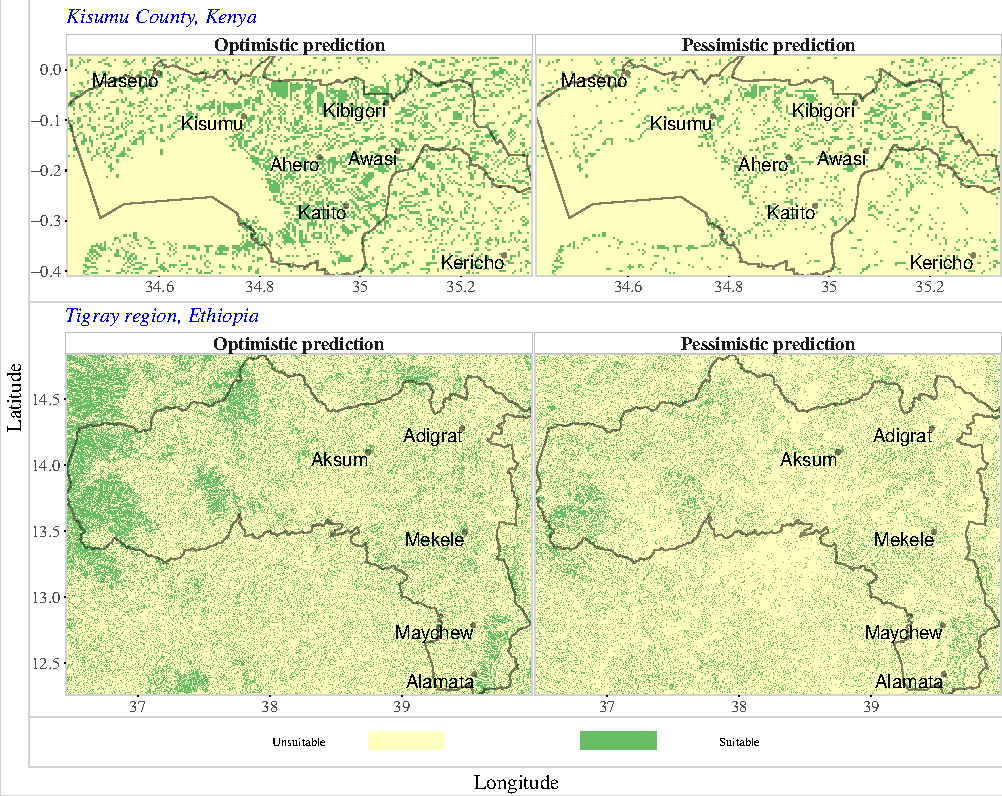
\includegraphics[width=1\linewidth,]{figures/Uncertainity_based_predictions_plot} 

}

\caption{Potential areas for FBFS based different level of uncertainities in Kisumu County, Kenya and Tigray region, Ethiopia.}\label{fig:fig10}
\end{figure}

\hypertarget{discussion}{%
\section{Discussion}\label{discussion}}

\hypertarget{conclusion}{%
\section{Conclusion}\label{conclusion}}

\hypertarget{refs}{}

\hypertarget{acknowledgements}{%
\section*{Acknowledgements}\label{acknowledgements}}
\addcontentsline{toc}{section}{Acknowledgements}

This study was jointly funded by the \href{https://www.daad.de/en/}{Deutscher Akademischer Austauschdienst} (German Academic Exchange Service; DAAD) and the \href{http://www.worldagroforestry.org/}{World Agroforestry Centre} (International Centre for Research in Agroforestry; ICRAF). We thank the farmers and experts who contributed in various ways during the development of the model. We thank the department of Dryland Agriculture of Mekelle University for guidance on the sampling frame in the Tigray region and for facilitating logistics during field work. Thanks to the participants of the leadership course in flood-based farming and water harvesting in Kenya and the participants of the International Training on Integrated Watershed Management and FBFS in Ethiopia, who drafted the models.

\hypertarget{references}{%
\section*{References}\label{references}}
\addcontentsline{toc}{section}{References}


\end{document}


